% !TEX root = ../main.tex
\section{Introduction}
\label{introduction}

There is overwhelming anecdotal evidence that data scientists spend at least
80\% of their time finding, preparing, integrating and cleaning data sets.
The remaining 20\% of their time is spent doing the actual desired analysis
tasks.
One data officer (Mark Schreiber
\eat{\mourad{Maybe, we should add him as a co-author?} }
of Merck) estimates the number is 98\%, in which case data
scientists spend less than one hour a week on tasks in their job description.

%----------------------------------
% Positioning Civilzer with respect to other systems early on
% to focus on dcv components more
%----------------------------------------

To address this problem, several systems and tools have been developed to for example,  to automate systematic transformations and data sources preparation for analytics (e.g., Data Wrangler System~\cite{2011-wrangler}, and the DataXFormer System~\cite{DBLP:conf/icde/AbedjanMIOPS16}); to integrate and unify large disparate data sources via schema mappings and record linkage exercises to help scientists work with data sets across silos (e.g., the Data Tamer System~\cite{DBLP:conf/cidr/StonebrakerBIBCZPX13}); or to extract facts and structured information from large corpora of text, images and other unstructured sources (e.g., DeepDive~\cite{DBLP:journals/pvldb/ShinWWSZR15}). However data scientists still face serious challenges when dealing with the large number of heterogeneous and ill-specified data sets in the enterprise data lake, where even the question of ''where to start looking?" is hard to answer. 

In this paper, we present the architecture of \dcv, a system under construction
at MIT, QCRI and Waterloo, whose main purpose  is to lower the ``mung work''  faced by
data scientists.  We present the main  design requirements of \dcv and the challenges it entails through use cases from the environment at Merck,  a large decentralized drug company with about XXX employees, of which YYY are data scientists.


{\bf[Discovery]} An exemplar data scientist at Merck would come up with a hypothesis, for example {\it the drug Ritalin causes brain cancer in rats weighing more than 1Kg}.  His first job is to first identify relevant data sets, both within and outside the Merck firewall that might contribute to testing this hypothesis.  Inside the firewall, Merck has in the order of  4,000 Oracle databases and countless other repositories.  A {\it Discovery} component in \dcv (cf. Section~\ref{sec:discovery}) has to assist the scientist with finding data sets of interest.

{\bf[Stitching]} The relevant data sets discovered by \dcv  are most likely  linked together by other intermediary data sets.  Hence, the next step is to construct ``data stitching'' paths among all of the data sets identified during discovery.  We discuss data stitching in detail when we discuss the {\it Data Stitcher} module in \dcv in Section~\ref{sec:stitching}. One can think of the output of the data stitcher as views on the underlying data sources. It is now necessary to perform data curation on these views by, for example, extracting data from source data storage systems, performing schema integration on the multiple views, transforming data into a common representation, cleaning erroneous values from the source data sets, and performing entity consolidation on resulting records. Multiple tools, such as Data Tamer, DataXFormer and the other example tools we mentioned earlier, can be used in tackling these curation and extraction challenges. We have recently evaluated some of the available cleaning tools on multiple data sets~\cite{evaluatioin} to identify the main challenges in this domain.

{\bf[Curating Polystore]} Since Merck has a variety of data storage systems and exascale data volumes, it is simply not reasonable to move all data to a  central data warehouse. Also, it is not economically, nor technically feasible  to perform data curation up front on the whole available enterprise data. Instead \dcv  must be a pull-based  system that perform stitching and data curation on demand, and  as data scientists need to access data to get
their work done.  Therefore, \dcv must be based on a polystore architecture~\cite{DBLP:journals/sigmod/DugganESBHKMMMZ15}, which  can pull data out of multiple underlying storage engines as needed and as dictated by the current analytics task.  Obviously, data cleaning, data transformation and entity consolidation must be integrated with querying the polystore.  In this way, a key technical optimization is to push filters and joins through cleaning operations and into the underlying data storage systems wherever possible.  The
merger of polystores and data curation steps is discussed in Section~\ref{sec:curating}, and we term the resulting system a {\it Curating Polystore}.  

{\bf[Cleanliness Estimation]}  Because of the human effort involved, the expensive processes of creating and curating materialized views during can be very disruptive to the human interaction experience (e.g., validating the view definitions and the stitching results, and validating the automatic cleaning decisions and suggestions).  Therefore, \dcv must estimate the cost of constructing and curating such materialized views  to reason about their feasibility within the scientists budget.  Estimating the cleanliness of a view  entails constructing a model for how dirty the data in the source data sets actually is, which we discuss in Section~\ref{sec:cleanliness}. An ancillary topic is to estimate the cleanliness that can be achieved for a given budget for cleaning activities.  In this way, a scientist can decide
whether or not he wishes to proceed with the project at hand.

{\bf [Optimizing Stitching]} It is highly inefficient and wasteful to  discard expensive-to-construct materialized views after their initial use by a data scientist.  Hence, we assume that they are generally retained for future use.  Moreover, future materialized views  may be based off previously constructed ones or on original data sources.  As a result, there may be several ways to construct a new view, with different  costs and accuracy. Therefore, the data stitching problem must be revisited to deal with this materialization cost/accuracy trade-off.  This is the subject of Sections~\ref{sec:enhancedstitching}.

{\bf [Handling Updates]}  If a source data set is updated, then
updates must be incrementally propagated through the data curation pipeline to
update downstream materialized views.  In some cases, the human effort involved may be
daunting, and the materialized view should be discarded rather than updated.  Lastly, if a
scientist updates a view, we must propagate changes to other derived views, as well as back upstream to data sources. Section~\ref{sec:updates} discusses the update issues and \dcv handles it.

{\bf [Workflow]} To have end-to-end functionality, \dcv has to offer a workflow engine whereby data scientists can iterate over our components in whatever order they wish; they can  undo previous workflow steps, and perform alternate branching from given materialized views. Section~\ref{sec:workflow} discusses the  workflow management in \dcv.

We describe the  current implementation of \dcv  in Section~\ref{sec:wild}, and indicate initial user experience in two use cases: the  MIT data warehouse and Merck. We conclude with final remarks and an  outline of  our future research plans in Section~\ref{sec:conclusion}.


\section{Architecture}

\dcv is a stack of modules that address three main tasks: {\em Discovery}, {\em
Linkage} and  {\em Polystore Query Processing}. Figure~\ref{fig:arch} shows the
general architecture of the \dcv system. The discovery layer to the underlying
slew of available data sets and data bases is what search engines are to the
internet; the module is responsible for taming the scale of the underlying
sources by defining data units of appropriate granularities, e.g., fields in
relations, with a high-performance \code{profiler}. When those profiles are
available, it finds relations such as schema or content similarity among them by
using the \code{graph builder} component. These relationships are then
represented in a data fabric similar in spirit to a knowledge graph
\cite{DBLP:conf/semweb/AuerBKLCI07,DBLP:conf/sigmod/BollackerEPST08,DBLP:conf/www/SuchanekKW07}.

The output graph is later used by the linkage layer to find more complex
relationship that allow stitching these units together to answer a wide range of
analytic queries against ad-hoc schemas. The linkage layer focuses primarily on
exploring the large space of possible ``join relationships'' that connect the
underlying data sets. For example, discovering (often fuzzy) Primary key-foreign
key relationship between tables with a \code{cleanliness estimator}. More
generally it extracts inclusion dependencies through the \code{FK-PK refiner},
which allow for joining or stitching these raw data sources together to populate
an analytics schema or a view. 

The query answering layer has the goal of answering queries posed by users.
Queries must be answered despite the heterogeneity and different levels of
trustworthiness and cleanliness of the underlying sources. This is possible
because the previous layer provide the capability of creating schema views
on-demand for the query to process by using the graph structure populated by
the discovery and linkage layer. To create the right view, a module
called \code{workflow orchestrator} is responsible for coordinating discovery
and linkage. After executing a query (\code{query processor}), the results will
be accompanied of certain quality, which can be improved by, for example,
performing some data cleaning on key tables that contribute to the results. The
module responsible for assessing the result quality and recommending improvement
strategies is called \code{quality controller}.

The three layers in \dcv have different scale and response time constraints,
which greatly affect the design and the choice of algorithms in each layer: The
discovery layer is ``always on'' working in the background to find, index and
mine connections among large number of data sets, hence, almost-linear
algorithms that work on a Big data scale is a key requirement. 
On the other hand, the linkage layer has to find more complex
relationships, such as inclusion dependencies, which are too expensive to run on
the full scale raw data. Hence, the linkage layer has to judiciously use the
graph output of the discovery layer to scope the search space. While the linkage
layer has an off-line component that focuses on mining these complex join
relationships, efficient use of the query submitted o the query processing layer
can help pruning the large space of possible join graphs. Finally, the polystore
query processing layer has the tightest response time constraints to respond
within reasonable time to ad-hoc analytics against often continuously changing
analytics schemas (views). Limiting the space of possible data stitching
strategies, while taking into account the polystore execution environment is a
key technical challenge. 

\begin{figure}
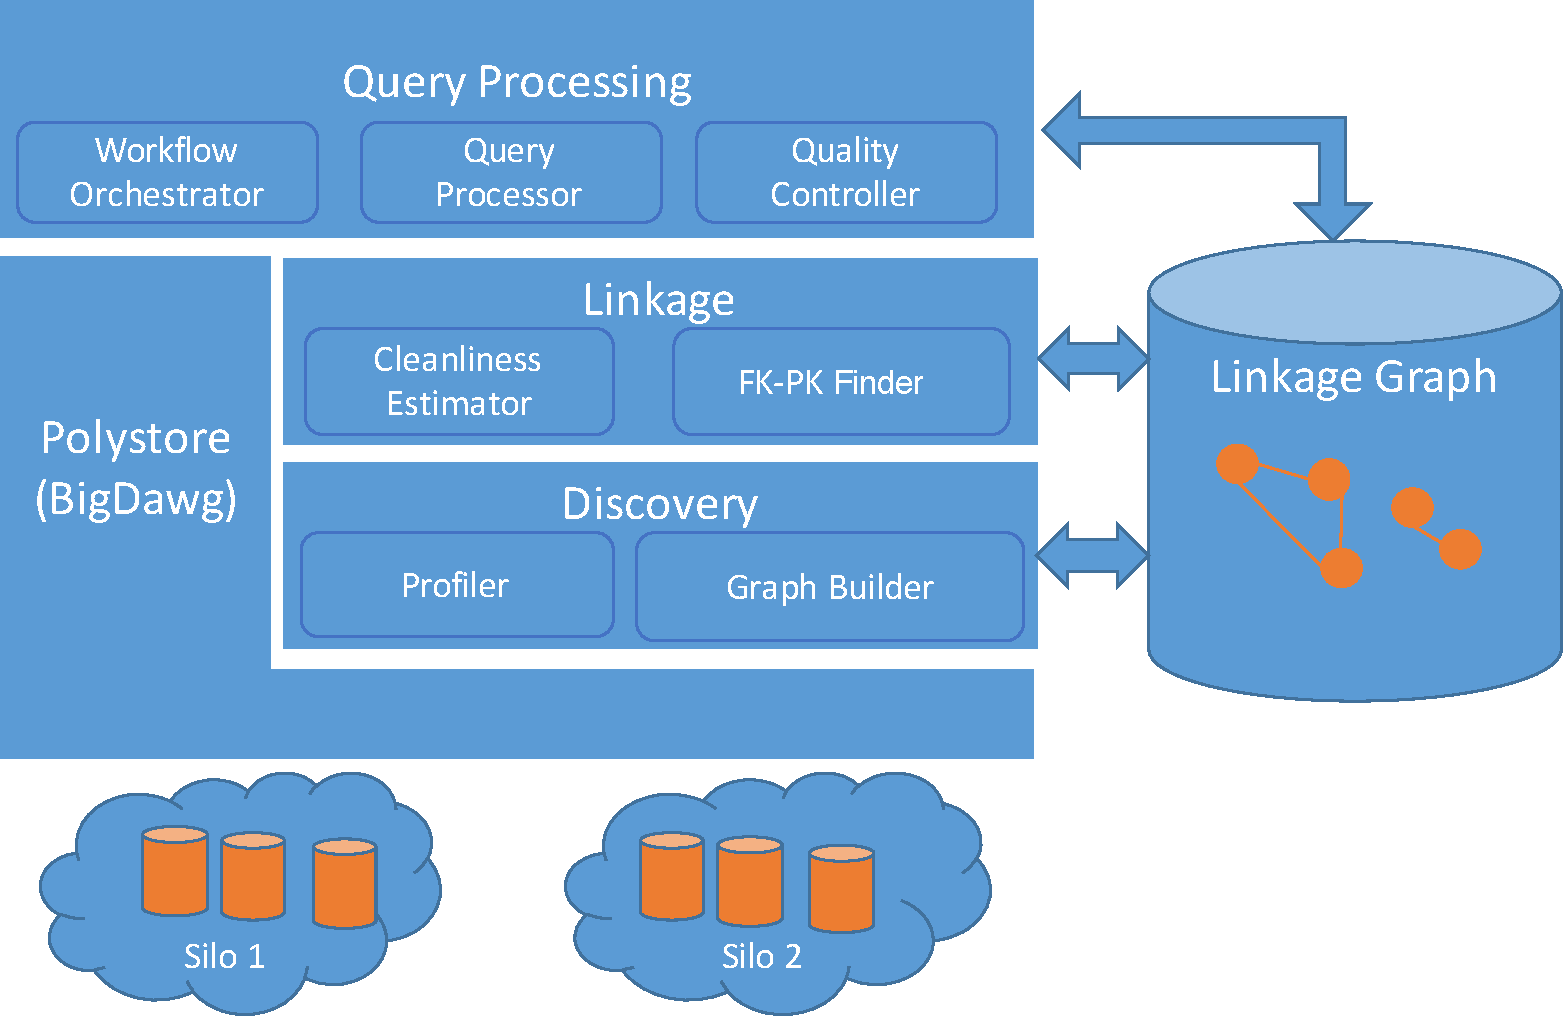
\includegraphics[width=3.5in]{arch3.pdf}
\caption{\dcv Architecture}
\label{fig:arch}
\end{figure}

\stab \nan{(3): We should merge the concepts of profiles, search path and
multigraph representation (Section 3), FK-PK (Section 4), and the join graph
(Section 6) here.}

%\subsection{\nan{\dcv Schema}}
%
%\nan{I would suggest to add here the global schema of \dcv. We need to
%emphasize the followings.}
%
%\stab \nan{(1): \dcv has a schema management module that is different from
%traditional ER-diagram. It has richer semantics. It is highly dynamic.}
%    
%\stab \nan{(2): If the above (1) is agreed, then in Figure 1, the ``Graph
%Builder'' should not be a part of Discovery. Instead, it should be, together
%with Linkage Graph, an independent module that supports all the others. I am
%thinking to change this module to be right above the data, but below all the
%other modules.}
%
%\nan{The other Sections can be significantly simplified then.}
